\documentclass[11pt, pdftex]{article}
\usepackage[margin=1in]{geometry}
\usepackage{graphicx}
\usepackage{amsmath}
\usepackage{listings}
\usepackage{semantic}
\usepackage[hyphens]{url}
\usepackage[breaklinks]{hyperref}
\usepackage[demo]{graphicx}
\usepackage{subcaption}
\usepackage{hyperref}
\title{Assignment (MiniProject) #3}
\author{Machiry Aravind Kumar}
\date{UCSB}
\begin{document}
\maketitle
\section{Dataset}
\subsection{Seeds Data Set}
This dataset is from UCI Archive: \url{https://archive.ics.uci.edu/ml/datasets/seeds}. Dataset contains various Geometric parameters of wheat kernels measured using a soft X-ray technique. It is non-destructive and considerably cheaper than other more sophisticated imaging techniques like scanning microscopy or laser technology. The problem is to classify these into one of the 3 different classes viz  Kama, Rosa and Canadian. For this Assignment, I selected samples for only 2 classes: Kama (Class label: 1) and Rosa (Class label: 2). Available Features in the dataset are:
\begin{itemize}
\item area A.
\item perimeter P.
\item compactness C.
\item length of kernel.
\item width of kernel,
\item asymmetry coefficient
\item length of kernel groove.
\end{itemize}
\section{Running SVM}
I used SVM package from $\texttt{sklearn}$ module. I used following kernel functions: $\texttt{linear,rbf}$ and   $\texttt{sigmoid}$ with different values of Penalty Parameter(C) which trades off misclassification of training examples against simplicity of the decision surface, in other words this parameter controls over fitting, larger value of C results in over fitting and Kernel coefficient (gamma) which defines how much influence a single training example has. Its clear that, we need to select a kernel function which gives highest accuracy with least C and gamma. The error rates (with 10-fold validation) of using different kernel functions with different C and gamma are as shown in Table \ref{tab:kerf}. I selected kernel function $\texttt{linear}$ with $C = 1.4$ and $gamma = 0$ as it gives the best result satisfying our constraints.
\begin{table}
\centering
\begin{tabular}{ | c | c | c | c |}
    \hline
    {\bf Kernel Function} & {\bf C} & {\bf gamma} & {\bf Mean Accuracy}\\ 
    \hline
    rbf & 0.1 & 0 & 50.0\\
	\hline
	sigmoid & 0.1 & 0 & 93.57\\
	\hline
	linear & 0.1 & 0 & 94.28\\
	\hline
	linear & 1 & 0 & 94.28 \\
	\hline
	linear & 1.1 & 0 & 94.42\\
	\hline
	linear & 1.2 & 0 & 95.0\\
	\hline
	linear & 1.3 & 0 & 95.71\\
	\hline
	{\bf linear} & {\bf 1.4} & {\bf 0} & {\bf 96.42}\\
	\hline
	linear & 1.5 & 0 & 96.42\\
	\hline
	linear & 10 & 0 & 96.42\\
	\hline
	\end{tabular}
	\caption{Effectiveness of various Kernel Functions}
    \label{tab:kerf}
\end{table}
\\
The results for different values of n are as shown in Table \ref{tab:svmcv}. The results are pretty accurate with 96.42$\%$ Accuracy and doesn't vary much with n, which proves that features are good for the classification. It also proves that a linear kernel with SVM is good fit for this classification problem.
\begin{table}
\centering
\begin{tabular}{ | c | c | c |}
    \hline
    {\bf N} & {\bf Mean Accuracy} & {\bf Mean Error}\\ 
    \hline
    3 & 94.98 & 5.01\\
	\hline
	4 & 95.00 & 5.00\\
	\hline
	5 & 94.28 & 5.71\\
	\hline
	6 & 94.26 & 5.73\\
	\hline
	7 & 95.00 & 5.00\\
	\hline
	8 & 94.89 & 5.10\\
	\hline
	9 & 94.95 & 5.04\\
	\hline
	10 & 96.42 & 3.57\\
	\hline
	11 & 95.74 & 4.25\\
	\hline
	\end{tabular}
	\caption{Cross Validation Results for Seeds Dataset using SVM with linear kernel}
    \label{tab:svmcv}
\end{table}
\section{LDF with gradient descent}
I implemented LDF with gradient descent where I used sigmoid function:$1/(1+e^{-y})$ as hypothesis to predict the value. Predicting class 2 if result is greater than or equal to 0.5 ( $>=$ 0.5) and Predicting class 1 otherwise. Using sigmoid function for hypotheses results in cost function as shown:

$-\frac{1}{m}\sum_{i=1}^{m}y^{i}\log(h_\theta(x^{i}))+(1-y^{i})\log(1-h_\theta(x^{i}))$
\\
\\
Another important reason to use sigmoid function as hypotheses rather than default $W^{T}X$ is because, {\bf the resulting cost function during computation of gradient descent using default method is non-convex thus resulting in various local minima and thus poor accuracy. Where as using sigmoid function results in cost function being convex resulting in global minima and good accuracy. The trend of cost function is as shown in Figure \ref{fig:costf}}
\\
\begin{figure}
    \centering
    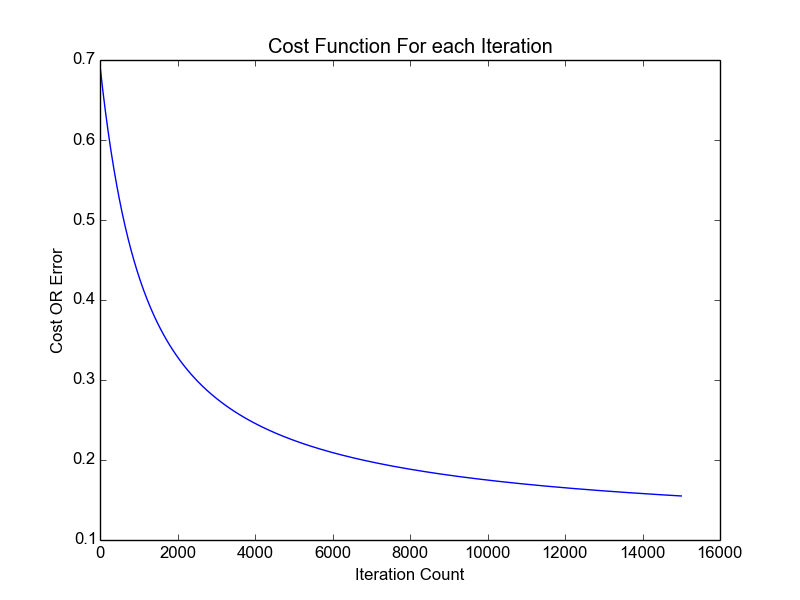
\includegraphics[width=0.6\textwidth]{pics/costf.png} 
    \caption{Cost Function Trend Against Iterations}
    \label{fig:costf}
\end{figure}
\\
With the above cost function, I used learning rate (i.e $\alpha$) of 0.0005 with regularization parameter (i.e $\lambda$) as 0.01 (to avoid over fitting) with 10,000 iterations. The core algorithm in python as shown below:

\begin{lstlisting}
for i in xrange(0, iters):

  theta_temp = self.theta
  
  #compute_hypothesis
  h_theta = self._sigmoid(numpy.dot(self.X, self.theta))
  
  #compute error
  diff = h_theta _ self.Y
  
  #update theta
  self.theta[0] = theta_temp[0] - self.learning_rate * \
     (1.0 / m) * sum(diff * self.X[:, 0])
  for j in xrange(1, n):
   val = theta_temp[
         j] _ self.learning_rate * (1.0 / m) * \
         (sum(diff * self.X[:, j]) + self.reg_param * m * theta_temp[j])
         
  self.theta[j] = val
\end{lstlisting}
\\
The complete code for this is present in file $\texttt{gradient\_descent.py}$. Cross validation results for various values of n is as shown in Table \ref{tab:gradcv}.\\
{\bf Weighted Vector computed using Gradient Descent is: [0.56232669359224408, 0.003148429546239455, 0.49146013233794189, 0.48967826722053615, 0.3474530090250722, 0.66867992711948321]}
\begin{table}
\centering
\begin{tabular}{ | c | c | c |}
    \hline
    {\bf N} & {\bf Mean Accuracy} & {\bf Mean Error}\\ 
    \hline
    3 & 96.40 & 3.59\\
	\hline
	4 & 96.42 & 3.57\\
	\hline
	5 & 95.00 & 5.00\\
	\hline
	6 & 94.98 & 5.01\\
	\hline
	7 & 95.00 & 5.00\\
	\hline
	8 & 94.24 & 5.75\\
	\hline
	9 & 94.21 & 5.78\\
	\hline
	10 & 94.28 & 5.71\\
	\hline
	11 & 94.11 & 5.88\\
	\hline
	\end{tabular}
	\caption{Cross Validation Results for Seeds Dataset using Gradient Descent}
    \label{tab:gradcv}
\end{table}

\end{document}